%%%%%%%%%%%%%%%%%%%%%%%%%%%%%%%%%%%%%%%%%
% The Legrand Orange Book
% LaTeX Template
% Version 2.1.1 (14/2/16)
%
% This template has been downloaded from:
% http://www.LaTeXTemplates.com
%
% Original author:
% Mathias Legrand (legrand.mathias@gmail.com) with modifications by:
% Vel (vel@latextemplates.com)
%
% License:
% CC BY-NC-SA 3.0 (http://creativecommons.org/licenses/by-nc-sa/3.0/)
%
% Compiling this template:
% This template uses biber for its bibliography and makeindex for its index.
% When you first open the template, compile it from the command line with the 
% commands below to make sure your LaTeX distribution is configured correctly:
%
% 1) pdflatex main
% 2) makeindex main.idx -s StyleInd.ist
% 3) biber main
% 4) pdflatex main x 2
%
% After this, when you wish to update the bibliography/index use the appropriate
% command above and make sure to compile with pdflatex several times 
% afterwards to propagate your changes to the document.
%
% This template also uses a number of packages which may need to be
% updated to the newest versions for the template to compile. It is strongly
% recommended you update your LaTeX distribution if you have any
% compilation errors.
%
% Important note:
% Chapter heading images should have a 2:1 width:height ratio,
% e.g. 920px width and 460px height.
%
%%%%%%%%%%%%%%%%%%%%%%%%%%%%%%%%%%%%%%%%%

%----------------------------------------------------------------------------------------
%	PACKAGES AND OTHER DOCUMENT CONFIGURATIONS
%----------------------------------------------------------------------------------------

\documentclass[11pt,fleqn]{book} % Default font size and left-justified equations

\usepackage{wasysym}
\usepackage{esint} % various fancy integral symbols
\usepackage{tikz}
\usepackage{tikz-3dplot}
\usepackage{pgfplots}
\pgfplotsset{compat=1.17}
\usetikzlibrary{patterns}
\usepackage{tkz-euclide} 

\usetikzlibrary {arrows.meta} 

\newcommand{\dd}{\mathrm{d}}
\newcommand{\div}{\mathrm{div}}
\newcommand{\rot}{\vv{\mathrm{div}}}
\newcommand{\grad}{\vv{\mathrm{grad}}}

\tikzset{
    support/.style={
        pattern=north east lines,
        draw=none,
        minimum width=0.3,
        minimum height=0.6
    }
    ,>=latex
}

\usepackage[d]{esvect}
%----------------------------------------------------------------------------------------

\input{structure} % Insert the commands.tex file which contains the majority of the structure behind the template

\begin{document}
%----------------------------------------------------------------------------------------
%	TITLE PAGE
%----------------------------------------------------------------------------------------

%\begingroup
%\thispagestyle{empty}
%\begin{tikzpicture}[remember picture,overlay]
%\coordinate [below=12cm] (midpoint) at (current page.north);
%\node at (current page.north west)
%{\begin{tikzpicture}[remember picture,overlay]
%\node[anchor=north west,inner sep=0pt] at (0,0) {
\includegraphics[width=\paperwidth]{background}}; % Background image
%\draw[anchor=north] (midpoint) node [fill=ocre!30!white,fill opacity=0.6,text opacity=1,inner sep=1cm]{\Huge\centering\bfseries\sffamily\parbox[c][][t]{\paperwidth}{\centering Cours de Physique-Chimie\\[15pt] % Book title
%{}\\[20pt] % Subtitle
%{\huge Lycée Baimbridge MP 2025-2026}}}; % Author name
%\end{tikzpicture}};
%\end{tikzpicture}
%\vfill
%\endgroup

%----------------------------------------------------------------------------------------
%	COPYRIGHT PAGE
%----------------------------------------------------------------------------------------

%\newpage
%~\vfill
%\thispagestyle{empty}

%\noindent Copyright \copyright\ CC BY 4.0 2025 Basile Poujol\\ % Copyright notice

%\noindent Licensed under the Creative Commons Attribution-NonCommercial 4.0 Unported License (the ``License''). You may not use this file except in compliance with the License. You may obtain a copy of the License at \url{http://creativecommons.org/licenses/by-nc/3.0}. See the License for the specific language governing permissions and limitations under the License.\\ % License information

%----------------------------------------------------------------------------------------
%	TABLE OF CONTENTS
%----------------------------------------------------------------------------------------

%\usechapterimagefalse % If you don't want to include a chapter image, use this to toggle images off - it can be enabled later with \usechapterimagetrue

\chapterimage{milky_way.jpeg} % Table of contents heading image

%\pagestyle{empty} % No headers

%\tableofcontents % Print the table of contents itself

%\cleardoublepage % Forces the first chapter to start on an odd page so it's on the right

%\pagestyle{fancy} % Print headers again



%\part{\'{E}lectromagnétisme}

\setcounter{chapter}{0}

\chapter{Gravitation}

La mécanique s'intéresse essentiellement à la description des mouvements d'objets solides.

La cause principale de ces mouvements, d'après la mécanique newtonienne, est la présence d'actions mécaniques. Nous avons vu en première année qu'il existe plusieurs types d'actions mécaniques :

Les forces qui s'exercent à distance. Par exemple :
\begin{itemize}
    \item La gravitation
    \item Les forces électrostatiques
    \item Les forces magnétiques
\end{itemize}

Les forces de contact, par exemple :
\begin{itemize}
    \item Une force de frottement fluide ou solide
    \item La réaction d'un support solide
    \item La tension d'un fil
    \item Le couple de torsion d'un fil
\end{itemize}

Après quelques rappels de dynamique du point, nous allons nous intéresser aux forces à distance. Dans ce chapitre, nous étudierons la force gravitationnelle, et dans un chapitre à venir nous nous intéresserons à la force électrique de Coulomb, qui présente des caractéristiques très similaires.

\section{Rappels de dynamique newtonienne du point}

Dans cette partie, nous allons revoir les principes de la mécanique classique qui ont été vus en première année. Ces principes sont tous équivalents puisqu'ils sont dérivés du principe fondamental de la dynamique :

\begin{theorem}
    Soit $M$ un point matériel soumis à un ensemble de forces $\vv F_{ext}$. Soit $\vv r = \vv{OM}$ le vecteur position du point $M$ dans un référentiel galiléen. Alors, l'accélération $\vv a$ du point $M$ dans ce référentiel est égale à la somme des forces extérieures qui lui sont appliquées :
    \begin{equation}
        m \frac{\dd² \vv r}{\dd t} = m \vv a = \sum \vv F_{ext}
    \end{equation}
\end{theorem}

Nous allons faire quelques rappels de ces principes de la mécanique à partir d'un problème très simple : le pendule.

\begin{figure}
    \centering

    \begin{tikzpicture}[scale=1.5]
       % Coordinates
        \coordinate (A) at (1.5,0);
        \coordinate (B) at (-1.5,0);
        \coordinate (C) at (0,2);
        % Axes
        \draw[->] (-2,2) -- (2,2) node[anchor=west]{$x$};
        \draw[->] (0,2) -- (0,-2) node[coordinate] (O){} node[anchor=north]{$z$};
        % Support
        \draw (-0.5,2) -- (0.5,2);
        \draw[support] (-0.5,2)  rectangle++ (1,0.25);
        % Coordinate markings (To draw angles and enclose vectors with dashed lines)
        \draw[->,white] (A) -- ++(270:1.25) node[coordinate] (R) {};
        \draw[->] (A) -- ++(306.8:1) node[coordinate] (P) {};
        % Lines and vectors
        \draw[dashed, gray] (C) -- ++(233.2:2.5);
        \draw (C) -- ++(306.8:2.5) node[midway,anchor=east]{$R$};
        \draw[dashed] (A) -- ++(306.8:1);
        \draw[->,ultra thick] (A) -- ++(126.8:0.7) node[anchor=east]{$\vv T$};
        \draw[->,ultra thick] (A) -- ++(270:1.) node[below]{$\vv P$};
        \draw[->] (A) -- ++(306.8:1) node[coordinate] (P) {} node[anchor=north]{$\vv{e_r}$};
        \draw[->] (A) -- ++(36:0.75) node[coordinate] (Q) {} node[anchor=south]{$\vv{e_\theta}$};
        % Angles
        \tkzMarkAngle[->, size=0.5,thick](O,C,A)
        \tkzLabelAngle[pos=0.7](O,C,A){$\theta$}

        \tkzMarkAngle[-, size=0.5,thick](R,A,P)
        \tkzLabelAngle[pos=0.7](R,A,P){$\theta$}
        % Pendulum trajectory
        \draw (-1.5,0) .. controls (-1,-0.5) and (1,-0.5) .. (1.5,0);
        % Circles
        \draw[fill = black] (A) circle (4pt) node[anchor=east]{$M$\,\,};
        \draw[fill = black] (C) circle (2pt) node[anchor=north west]{$O$};
        \draw[dashed] (B) circle (4pt); 
    \end{tikzpicture}

    \caption{Le problème du pendule simple. Schéma adapté à partir d'un schéma de Gabriel Pereira Coelho.}
    \label{fig:pendule}
\end{figure}

\subsection{Principe fondamental de la dynamique}

\begin{capex}
	Etablir l'équation du mouvement correspondant aux petites oscillations du pendule à l'aide du principe fondamental de la dynamique.
\end{capex}

%Nous avons déjà énoncé le principe plus haut. Nous nous plaçons dans le référentiel terrestre, supposé galiléen. Le pendule est soumis à :
%\begin{itemize}
%    \item La force de tension du fil $\vv T$, orientée selon $-\vv{e_r}$ et qui le contraint à rester à l'intérieur d'un cercle de rayon $R$;
%    \item Son poids $\vv P = m \vv g$, dirigé vers le bas selon $+ \vv{e_z}$.
%\end{itemize}
%La vitesse du point $M$ dans le référentiel s'écrit :
%\begin{equation}
%    \vv v = r \dot{\theta} \vv{e_\theta}
%\end{equation}
%Par ailleurs :
%\begin{equation}
%    \frac{\dd \vv{e_\theta}}{\dd t} = - \dot{\theta} \vv{e_r}
%\end{equation}
%Si bien que l'accélération s'écrit :
%\begin{equation}
%    \frac{\dd \vv v}{\dd t} = r \ddot{\theta} \vv{e_\theta} - r \dot{\theta}² \vv{e_r}
%\end{equation}
%On projette le principe fondamental de la dynamique selon $\vv e_\theta$ pour obtenir :
%\begin{equation}
%    m R \ddot \theta = - m g \sin \theta
%\end{equation}
%En notant $\omega = \sqrt{g/R}$ et en utilisant l'approximation des petits angles on obtient l'équation de l'oscillateur harmonique :
%\begin{equation}
%    \ddot \theta + \omega² \theta = 0
%\end{equation}
%dont la solution est un mouvement sinusoïdal :
%\begin{equation}
%    \theta(t) = \theta_0 \sin(\omega t + \varphi)
%\end{equation}
%où $\theta_0$ et $\phi$ dépendent des conditions initiales de vitesse et de position.

\subsection{Théorème du moment cinétique}

Il est également possible de résoudre ce problème à partir du théorème du moment cinétique. Le théorème est donné par :
\begin{theorem}[Théorème du moment cinétique]
    Soit $M$ un point matériel de masse $m$ soumis à un ensemble de forces $\vv F_{ext}$. Dans un référentiel galiléen dans lequel le point $O$ est fixe, la variation du moment cinétique $\vv{L_O}$ du point $M$ par rapport au point $O$ est vaut :
    \begin{equation}
        \frac{\dd \vv{L_O}}{\dd t} = \sum \mathcal{M}_0 ( \vv F_{ext} )
    \end{equation}
\end{theorem}

\begin{capex}
	Retrouver l'équation du mouvement à partir du théorème du moment cinétique.
\end{capex}

%Nous l'appliquons ici au pendule simple. Le moment cinétique du pendule par rapport au point $O$ s'écrit :
%\begin{equation}
%    \vv L_O = \vv{OM} \wedge m \vv v = R \vv{e_r} \wedge m R \dot \theta \vv{e_\theta} = m R² \dot \theta \vv{e_y}
%\end{equation}
%Par ailleurs, le moment de la force de tension est nul (elle est orientée selon l'axe $(OM)$) et le moment du poids est donné par :
%\begin{equation}
%    \mathcal{M}_O(\vv P) = \vv{OM} \wedge mg \vv{e_z} = - m R g \sin \theta \vv{e_y}
%\end{equation}
%En appliquant le théorème du moment cinétique, on obtient :
%\begin{equation}
%    m R² \ddot \theta = - m R g \sin \theta
%\end{equation}
%Et l'on retrouve l'équation du mouvement :
%\begin{equation}
%    R \ddot \theta + g \sin \theta = 0
%\end{equation}
%La suite du raisonnement est identique au cas où l'on a appliqué le PFD.

\subsection{Energétique}

On peut enfin utiliser la conservation de l'énergie du pendule, qui est un caps particulier du théorème de l'énergie mécanique :

\begin{theorem}[Conservation de l'énergie]
    Soit $M$ un point matériel de masse $m$, soumis uniquement à des forces conservatives qui dérivent d'une énergie potentielle $E_p$, et des forces qui ne travaillent pas. Alors son énergie mécanique est constante :
    \begin{equation}
        E_m = E_c + E_p = \mathrm{constante}
    \end{equation}
\end{theorem}

\begin{capex}
	Retrouver l'équation du mouvement du pendule en utilisant la conservation de l'énergie.
\end{capex}

%En effet, l'énergie cinétique du pendule s'écrit :
%\begin{equation}
%    E_c = \frac{1}{2} m {\vv v}² = \frac{1}{2} m R² {\dot \theta}² 
%\end{equation}
%Son énergie potentielle de pesanteur s'écrit :
%\begin{equation}
%    E_p = m g z = - m g R \cos \theta
%\end{equation}
%Par ailleurs, la force de tension est perpendiculaire au mouvement, elle ne travaille donc pas.
%La conservation de l'énergie implique que :
%\begin{equation}
%    E_m = E_c + E_p = \frac{1}{2} m R² {\dot \theta}^2 - m g R \cos \theta = \mathrm{constante}
%\end{equation}
%En dérivant cette équation par rapport au temps, on obtient alors :
%\begin{equation}
%    m R² \dot \theta \ddot \theta + m g R \dot \theta \sin \theta = 0
%\end{equation}
%ou encore, après simplification :
%\begin{equation}
%    R \ddot \theta + g \sin \theta = 0
%\end{equation}

\begin{encart}[Pendule et sismomètre]
    Le pendule simple est un système qui a été largement discuté en physique classique et permet d'appliquer de manière simple de nombreuses théories. Mais il a aussi un certain nombre d'applications techniques.

    En particulier, les sismomètres fonctionnent à l'aide d'un mécanisme de pendule simple pour mesurer les mouvements horizontaux du sol. La mesure de la position du pendule se faisait auparavant à l'aide d'un stylo qui écrivait sur une feuille de papier. Depuis récemment, elle a été remplacée par les sismomètres optiques, dans lesquels la position du pendule est mesurée par interférométrie laser. En 2020, un sismomètre optique a été installé notamment au sommet de la Soufrière pour surveiller l'activité volcanique.
\end{encart}

\begin{figure}
    \centering
    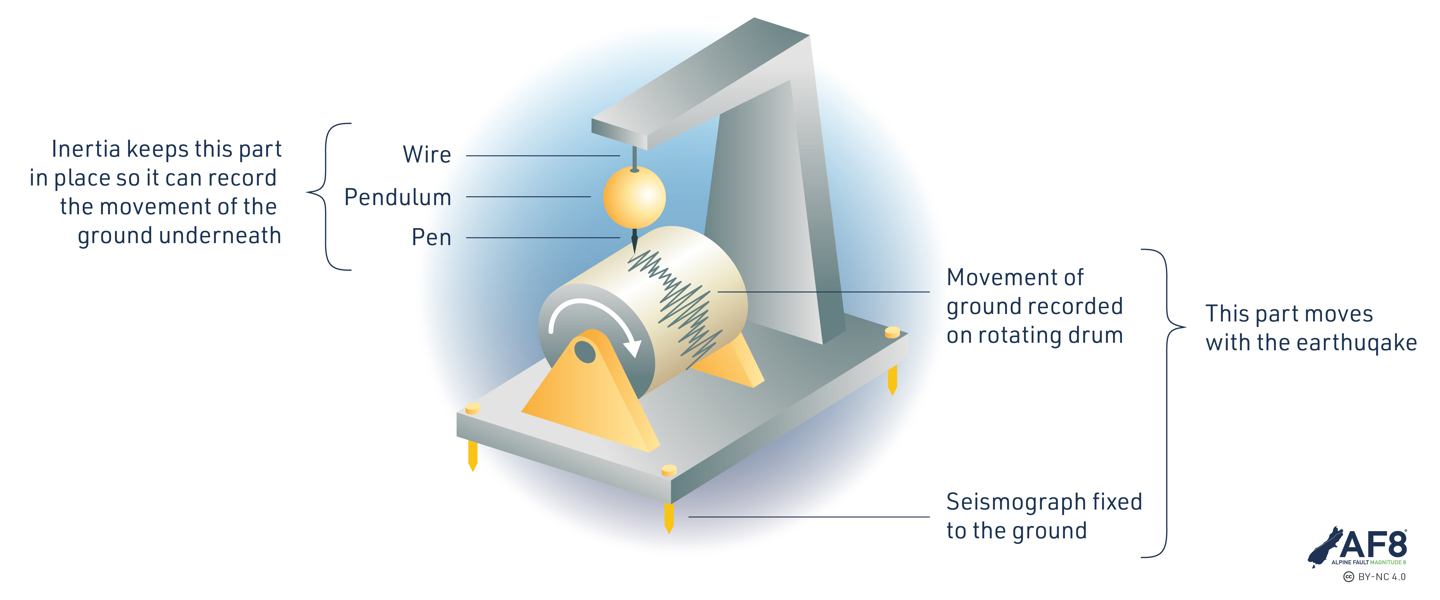
\includegraphics[width=\linewidth]{Pictures/sismographe.jpg}
    \caption{Principe de fonctionnement d'un sismomètre à pendule. Source : Alpine Fault M8.}
    \label{fig:sismographe}
\end{figure}

\section{Rappels sur la gravitation}

Nous allons maintenant nous intéresser à la force de gravitation. Cette force est une interaction à distance, attractive, qui concerne deux objets massifs. Elle est donnée par la loi de la gravitation universelle :

\begin{theorem}[Loi de la gravitation universelle]
    Soient deux corps massifs $M_1$ et $M_2$ de masses respectives $m_1$ et $m_2$. Ces deux corps s'attirent mutuellement par une force d'interaction donnée par :
    \begin{equation}
        \vv F_{1 \rightarrow 2} = - G \frac{m_1 m_2}{||\vv{M_1 M_2}||^2} \frac{\vv{M_1 M_2}}{||\vv{M_1 M_2}||}
    \end{equation}
    où $G = 6.67\times10^{-11}$m$^3 \cdot$kg$^{-1}\cdot$s$^{-2}$ est la constante de gravitation universelle.
\end{theorem}

Deux propriétés fondamentales de la force de gravitation ont été vues en 1e année :
\begin{itemize}
    \item La force de gravitation est une force conservative. Dans le cas où la force de gravitation est exercée par une masse ponctuelle, elle dérive d'un potentiel, appelé potentiel gravitationnel :
    \begin{equation}
        V = -G \frac{m_1 m_2}{r}
    \end{equation}
    \item Il s'agit d'une force centrale. En particulier, le moment de cette force par rapport au point où se trouve l'objet massif qui exerce la force est nul.
\end{itemize}

\subsection{Forces centrales conservatives}

Plusieurs propriétés importantes des forces centrales et/ou conservatives ont été vues en première année. Ces propriétés sont évidemment au programme du concours, et il est essentiel d'y passer plus de temps pendant vos révisions des écrits. Dans cette partie, un petit résumé est présent qui vous aidera à réviser avant le concours et vous permet de faire le lien entre les programmes de 1e et 2e année. \textbf{Ce résumé ne se substitue pas à votre cours de première année}, pour lequel de nombreux chapitres sont dédiés à la mécanique.

\paragraph{Force centrale}

\begin{definition}
    Une force centrale est une force dont le support passe par un point fixe $O$ dans le référentiel d'étude.
\end{definition}

\begin{proposition}[Mouvement plan]
    Si un point matériel $M$ est soumis à une force centrale dans un référentiel galiléen, alors le mouvement de $M$ est plan et orthogonal au moment cinétique de $M$ par rapport à $O$.
\end{proposition}

\begin{demonstration}
    Soit $M$ un point matériel de masse $m$ et de vistesse $\vv v$ soumis à une force centrale dans un référentiel galiléen. Le moment de la force centrale par rapport au point $O$ étant nul (par définition de la force centrale), on en déduit, par le théorème du moment cinétique, que le moment cinétique de $M$ par rapport à $O$ est constant :
    \begin{equation}
        \vv L_O = \vv{OM} \wedge m \vv v = \vv{\mathrm{constante}}
    \end{equation}
    En tout instant, nous avons $\vv{OM} \wedge \vv L_O = \vv 0$, et donc $M$ est contenu dans le plan passant par $O$ et normal à $\vv L_O$. Comme $\vv L_O$ est un vecteur constant, ce plan est toujours le même et le mouvement du point $M$ est contenu dans ce plan. 
\end{demonstration}

\begin{proposition}[Loi des aires]
    Soit $M$ un point matériel soumis à une force centrale. Le mouvement étant plan, nous pouvons nous placer dans un repère de coordonnées polaires $(r,\theta)$ dans le plan du mouvement, tel que la force centrale soit orientée selon $\pm \vv{e_r}$. Alors :
    \begin{itemize}
        \item La quantité $C = r^2 \dot \theta$ est constante et est appelée constante des aires ;
        \item L'aire $\dd \mathcal{A}$ balayée par $\vv{OM}$ pendant $\dd t$ est donnée par :
        \begin{equation}
            \dd \mathcal{A} = \frac{C}{2} \dd t
        \end{equation}
    \end{itemize}
\end{proposition}

\begin{demonstration}
    Soit $M$ un point matériel soumis à une force centrale. Nous nous plaçons dans le système de coordonnées polaires d'origine $O$ et de coordonnées $(r,\theta)$ situé dans le plan du mouvement. Dans ce système, le moment cinétique s'écrit :
    \begin{equation}
        \vv L_O = \vv{OM} \wedge m \vv v = m r^2 \dot \theta \vv{e_z}
    \end{equation}
    Comme il s'agit d'un vecteur constant, alors $C = r^2 \dot \theta$ est constant.

    Par ailleurs, l'aire balayée par $\vv{OM}$ pendant $\dd t$ est donnée par :
    \begin{equation}
        \dd \mathcal{A} = \frac{1}{2} || \vv{OM} \wedge \dd \vv{OM} || = \frac{1}{2} || r \vv{e_r} \wedge r \dot \theta \dd t \vv{e_\theta} || = \frac{r^2 \dot \theta}{2} \dd t = \frac{C}{2} \dd t 
    \end{equation}
\end{demonstration}

\paragraph{Force centrale conservative}

\begin{proposition}
    Soit $\vv F$ une force centrale conservative qui dérive d'une énergie potentielle $E_p(r)$. On se place dans le repère de coordonnées polaires $(r,\theta)$ d'origine $O$ dans le plan du mouvement.

    Alors l'énergie mécanique de $M$ peut s'écrire comme la somme d'une énergie cinétique radiale et d'une énergie potentielle efficace :
    \begin{equation}
        E_m = E_{p,eff} + \frac{1}{2} m {\dot r}^2
    \end{equation}
    où
    \begin{equation}
        E_{p,eff}(r) = \frac{1}{2} m \frac{C^2}{r^2} + E_p(r)
    \end{equation}
    où $C$ est la constante des aires. L'étude du mouvement selon $\vv{e_r}$ peut donc se résumer à l'étude classique du mouvement unidimensionnel d'un point selon la coordonnée $r$ avec une énergie potentielle efficace $E_{p,eff}$.
\end{proposition}

\begin{demonstration}
    L'énergie cinétique du système est donnée par :
    \begin{equation}
        E_c = \frac{1}{2} m {\vv v}^2 = \frac{1}{2} m (\dot r^2 + r^2 \dot \theta^2) = \frac{1}{2} m \dot r^2 + \frac{1}{2} m \frac{C^2}{r^2}
    \end{equation}
    On constate que le second terme ne dépend que de la position $r$ et pas de la vitesse de la particule $M$, si bien que l'on peut simplement étudier le mouvement comme un mouvement unidimensionnel selon $r$ avec une énergie potentielle efficace $E_{p,eff}(r)$ donnée par le second terme de l'énergie cinétique.
\end{demonstration}

\section{Champ gravitationnel}

Supposons qu'un corps massif de masse $m_0$ se trouve à l'origine $O$ d'un repère en coordonnées sphériques. Soit un autre corps de masse $m$ localisé au point $M(\vv r)$. Ce corps est soumis à une force :
\begin{equation}
    \vv F = - G \frac{m_0 m}{r^2} \vv{e_r}
\end{equation}
On constate que cette force est proportionnelle à la masse du corps qui subit la force, et que le facteur de proportionnalité ne dépend que de l'emplacement. Ceci nous permet de définir le concept de champ gravitationnel :
\begin{definition}[Champ gravitationnel]
    Le champ gravitationnel, noté $\vv{\mathcal{G}}(\vv r)$, est la force gravitationnelle que subirait une particule ponctuelle de masse unité placée au point $\vv r$.  Une particule de masse $m$ se trouvant dans un champ gravitationnel $\vv{\mathcal{G}}$ subit alors une force gravitationnelle $\vv F = m \vv{\mathcal{G}}$.
\end{definition}

\begin{capex}
	Etablir l'expression, puis calculer la valeur numérique, du champ gravitationnel à la surface de la Terre, noté $\vv g$. On donne le rayon et la masse de la Terre : $R_T = 6380$\,km et $M_T = 5.97 \cdot 10^{24}$\,kg.
\end{capex}

Ce calcul se généralise en tout point de l'espace situé à l'extérieur de l'astre considéré :
\begin{proposition}
    Le champ gravitationnel produit par une masse ponctuelle $m$ située à l'origine $O$ d'un repère sphérique de coordonnées $(r,\theta,\varphi)$ est donné par la relation :
    \begin{equation}
        \vv{\mathcal{G}} = - \frac{G m}{r^2} \vv{e_r}
    \end{equation}
\end{proposition}

A la différence de la force de gravitation, qui n'existe que si un objet est présent pour la subir, le champ gravitationnel est toujours défini en tout point de l'espace, même dans le vide. Ceci nous permet de définir des outils permettant de le visualiser, en particulier les lignes de champ.

\begin{definition}[Lignes de champ]
    Une ligne de champ gravitationnel est une ligne parallèle en tout point au vecteur champ gravitationnel $\vv{\mathcal{G}}$. Les lignes de champ sont orientées dans le sens du champ gravitationnel, c'est à dire vers les objets massifs.
\end{definition}

\begin{figure}
    \centering
    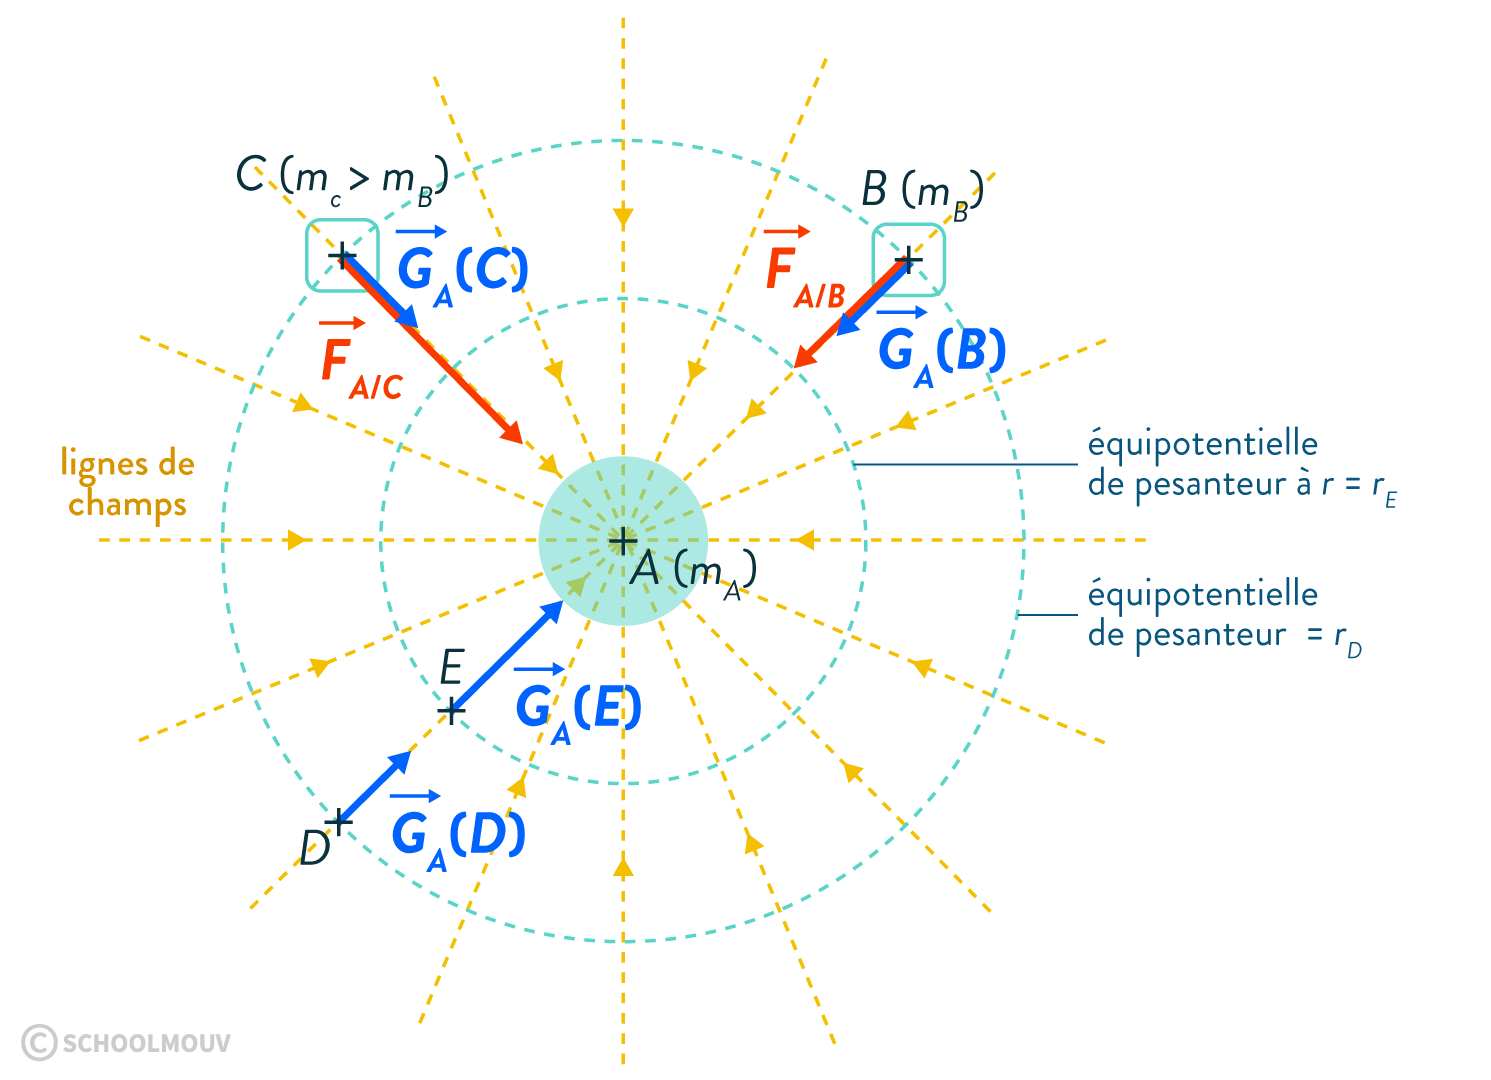
\includegraphics[width=0.75\linewidth]{Pictures/champ_gravitationnel_masse_ponctuelle.png}
    \caption{Lignes de champ produites par une masse ponctuelle. Le vecteur champ gravitationnel est indiqué en plusieurs points. Il est colinéaire aux lignes de champ et plus intense au voisinage de la masse. Deux équipotentielles sont également représentées, ce concept est défini plus tard.}
    \label{fig:champ_masse_ponctuelle}
\end{figure}

\begin{example}[Lignes de champ produites par une masse ponctuelle]
    Nous avons vu que le champ gravitationnel produit par une masse ponctuelle $m$ est donné, dans le repère sphérique approprié, par la relation :
    \begin{equation}
        \vv{\mathcal{G}} = - \frac{G m}{r^2} \vv{e_r}
    \end{equation}
    En tout point de l'espace, $\vv{\mathcal{G}}$ est colinéaire au vecteur unitaire $\vv{e_r}$ et orienté vers l'intérieur, ainsi les lignes de champ sont des demi-droites partant de l'origine et orientées vers l'intérieur.
\end{example}

\subsection{Additivité du champ}

La force gravitationnelle est proportionnelle à la masse de l'objet qui subit la force, ce qui nous a permis de définir le champ gravitationnel. Mais elle est également proportionnelle à la masse de l'objet qui produit la force. Ceci nous permet d'exploiter la propriété d'additivité du champ :

\begin{proposition}[Additivité du champ]
    Le champ gravitationnel produit par deux objets massifs est la somme des champs produits individuellement par chacun de ces objets. 
\end{proposition}

\section{Potentiel gravitationnel}

Calculons le travail de la force gravitationnelle le long de la trajectoire d'une masse ponctuelle $m$ parcourant un chemin $\Gamma$. Nous pouvons découper ce chemin en éléments infinitésimaux $\vv{\mathrm{d} l}$ définis comme :
\begin{equation}
	\vv{\mathrm{d}l} = \mathrm{d}x \vv{e_x} + \mathrm{d}y \vv{e_y} + \mathrm{d}z \vv{e_z}
\end{equation}
Le travail élémentaire exercé par la force gravitationnelle sur la particule le long de ce déplacement est donné par:
\begin{equation}
    \delta W = \vv F \cdot \mathrm{d} \vv l = m \vv{\mathcal{G}} \cdot \mathrm{d} \vv l
\end{equation}
si bien que le travail de la force le long d'un chemin macroscopique $\Gamma$ s'écrit:
\begin{equation}
    W = \int_\Gamma  m \vv{\mathcal{G}} \cdot \mathrm{d} \vv l
\end{equation}

Cette intégrale correspond à ce que l'on nomme la circulation du champ gravitationnel :

\begin{definition}
    La circulation d'un champ vectoriel $\vv A$ le long d'un chemin $\Gamma$ correspond à l'intégrale du champ le long de ce chemin :
    \begin{equation}
        \mathcal{C} = \int_\Gamma \vv A \cdot \mathrm{d}\vv l
    \end{equation}
\end{definition}

\begin{example}
    Calculons le travail issu du déplacement d'une particule $M$ de masse $m$ au voisinage d'une particule charge $m_0$ située sur l'origine. La particule $M$ est soumise à la force gravitationnelle et on a:
    \begin{align}
        W &= \int_\Gamma  m \vv{\mathcal{G}} \cdot \mathrm{d} \vv l \\
        &= \int_\Gamma G \frac{m m_0}{r^2} \vv{e_r} \cdot \mathrm{d} \vv l\\
        &=  G m m_0 \int_\Gamma \frac{\mathrm{d}r}{r^2} \\
        &= G m m_0 \left(\frac{1}{r_2} - \frac{1}{r_1} \right)
    \end{align}
\end{example}
On constate que le travail de la force électrostatique ne dépend que de la position initiale et de la position finale de la particule, données par $r_1$ et $r_2$: il est indépendant du chemin suivi pour relier ces deux positions. On en déduit que la force gravitationnelle est une force conservative :

\begin{proposition}[Conservativité de la force électrique]
    La force gravitationnelle est une force \textbf{conservative}.
\end{proposition}

La force gravitationnelle dérive donc d'un potentiel, en effet il est possible d'écrire son travail comme une différence d'énergie potentielle gravitationnelle :
\begin{equation}
    W = E_{pot, 1} - E_{pot,2}
\end{equation}
avec
\begin{equation}
    E_{pot} = -\frac{G m m_0}{r} + C
\end{equation}
$C$ est une constante que l'on prend généralement égale à zéro afin d'avoir une énergie potentielle nulle loin de tout corps massif ($r \to \infty$).

\begin{definition}[Potentiel gravitationnel]
    On définit le potentiel gravitationnel $\Phi$ comme l'énergie potentielle gravitationnelle par unité de masse. L'énergie potentielle gravitationnelle d'une masse ponctuelle de masse $m$ s'écrit alors:
    \begin{equation}
        E_{pot} = m \Phi
    \end{equation}
    Il se mesure en Joules par kilogramme (J/kg).
\end{definition}

Pour visualiser le potentiel électrique, on dessine souvent des surfaces équipotentielles (ou lignes équipotentielles si le problème est à deux dimensions):
\begin{definition}
    Une surface équipotentielle est une surface sur laquelle le potentiel gravitationnel a une valeur constante.
\end{definition}

\subsection{Opérateur gradient et lien entre potentiel et champ}

Nous cherchons maintenant à relier le potentiel gravitationnel et le champ gravitationnel par une relation directe, sans faire intervenir d'intégrale. Pour cela, nous pouvons remarquer que
Le travail élémentaire de la force électrique le long d'un chemin $\mathrm{d} \vv l$ peut s'écrire d'une part:
\begin{equation}
    \delta W = -\mathrm{d}E_{pot} = - m \mathrm{d} \phi
\end{equation}
et d'autre part:
\begin{equation}
    \delta W = m \vv{\mathcal{G}} \cdot \mathrm{d} \vv l
\end{equation}

\paragraph{Cas à une dimension}
Dans le cas d'un problème à une dimension, où $x$ est la seule coordonnée d'espace, alors $\vv{\mathcal{G}}  = \mathcal{G} \vv{e_x}$, $\vv{\dd \ell} = \dd x \vv{e_x}$ nous pouvons écrire $\vv{\mathcal{G}} \cdot \mathrm{d} \vv l = \mathcal{G} \dd x$. On obtient alors une relation reliant le champ de gravitation et le potentiel gravitationnel :
\begin{equation}
    \mathcal{G} = - \frac{\dd \phi}{\dd x}
\end{equation}

\paragraph{Cas à plusieurs dimensions}
En réalité, l'espace a plusieurs dimensions. Nous voudrions remplacer l'expression :
\begin{equation}
    \mathrm{d} \phi = - \vv{\mathcal{G}} \cdot \vv{\dd \ell}
    \label{eq:dphi}
\end{equation}
par une relation du type "$\vv{\mathcal{G}} = \frac{\dd \phi}{\vv{\dd \ell}}$". Mais cette relation est évidemment fausse puisqu'on ne peut pas diviser un scalaire par un vecteur !

Pour obtenir cette relation, nous décomposons comme suit l'équation \ref{eq:dphi}:
\begin{equation}
    \mathrm{d} \phi = - (\mathcal{G}_x \dd x + \mathcal{G}_y \dd y + \mathcal{G}_z \dd z)
\end{equation}
ce qui se traduit immédiatement par :
\begin{equation}
    \mathcal{G}_x = \frac{\partial \phi}{\partial x} \quad ; \quad \mathcal{G}_y = \frac{\partial \phi}{\partial y} \quad ; \quad \mathcal{G}_z = \frac{\partial \phi}{\partial z} 
\end{equation}

Nous allons simplifier cette équation en introduisant l'opérateur gradient.

\begin{definition}[Opérateur gradient]
    L'opérateur gradient, noté $\grad$, est un opérateur \textbf{vectoriel} défini par son action sur un champ \textbf{scalaire} $A$ :
    \begin{equation}
        \grad(A) = \frac{\partial A}{\partial x} \vv{e_x} + \frac{\partial A}{\partial y} \vv{e_y} + \frac{\partial A}{\partial z} \vv{e_z}
    \end{equation}
\end{definition}

\begin{remark}
    Il existe une autre notation pour la gradient, utilisant le vecteur nabla :
    \begin{equation}
        \vv \nabla = \frac{\partial}{\partial x} \vv{e_x} + \frac{\partial}{\partial y} \vv{e_y} + \frac{\partial}{\partial z} \vv{e_z}
    \end{equation}
    On note alors $\grad(A) = \vv \nabla A$. Cette notation est la notation officielle internationale. La notation $\grad$ est la notation française, qui figure au programme et est utilisée dans la plupart des concours.
\end{remark}


L'une des propriétés fondamentales de l'opérateur gradient est le théorème du gradient :
\begin{theorem}[Théorème du gradient]
    Soit $\Gamma$ un contour reliant deux points $M_1$ et $M_2$, et soit $A$ un champ scalaire défini le long de ce contour. Alors :
    \begin{equation}
        \int_\Gamma \grad(A) \cdot \vv{\dd \ell} = A(M_2) - A(M_1)
    \end{equation}
\end{theorem}

\begin{demonstration}
    Nous apouvons écrire la différentielle du champ $A$ :
    \begin{equation}
        \dd A = \frac{\partial A}{\partial x} \dd x + \frac{\partial A}{\partial y} \dd y + \frac{\partial A}{\partial z} \dd z 
    \end{equation}
    On reconnaît ici le produit scalaire entre le gradient de $A$ et le vecteur élémentaire $\vv{\dd \ell}$. On obtient alors :
    \begin{equation}
        \dd A = \grad(A) \cdot \vv{\dd \ell}
    \end{equation}
    On intègre le long du contour et on obtient :
    \begin{equation}
        \int_\Gamma \grad(A) \cdot \vv{\dd \ell} = \int_\Gamma \dd A = A(M_2) - A(M_1)
    \end{equation}
\end{demonstration}

\paragraph{Retour au lien entre potentiel gravitationnel et champ gravitationnel}

Maintenant que nous avons introduit l'opératuer gradient, nous obtenons un lien direct entre champ gravitationnel et potentiel gravitationnel :

\begin{proposition}
    Le champ gravitationnel est le gradient du potentiel gravitationnel:
    \begin{equation}
    \vv{\mathcal{G}} = -\vv{\mathrm{grad}}(\Phi)
    \end{equation}
\end{proposition}

\begin{demonstration}
Le travail élémentaire de la force gravitationnelle le long d'un chemin $\mathrm{d} \vv \ell$ peut s'écrire d'une part:
\begin{equation}
    \delta W = \vv{\mathcal{G}} \cdot \mathrm{d} \vv \ell
\end{equation}
et d'autre part:
\begin{equation}
    \delta W = -\mathrm{d}E_{pot} = - m \mathrm{d} \phi = - m\,\vv{\mathrm{grad}}(\phi) \cdot \mathrm{d} \vv \ell
\end{equation}
par propriété de l'opérateur gradient. Par identification, on en déduit:
\begin{equation}
    \vv{\mathcal{G}} \cdot \mathrm{d} \vv l = -\vv{\mathrm{grad}}(\phi) \cdot \mathrm{d} \vv l
\end{equation}
Ceci étant vrai pour tout élément $\mathrm{d} \vv l$ on en déduit que:
\begin{equation}
    \vv{\mathcal{G}} = -\vv{\mathrm{grad}}(\phi)
\end{equation}
\end{demonstration}

Une conséquence de cette relation est la propriété géométrique suivante :
\begin{proposition}
    Les surfaces équipotentielles et les lignes de champ sont orthogonales.
\end{proposition}
Par ailleurs, il est possible de relier l'intensité du champ gravitationnel à la distance entre les surfaces équipotentielles :
\begin{proposition}
    Le champ gravitationnel est d'autant plus intense que les surfaces équipotentielles sont rapprochées.
\end{proposition}

Pour une masse ponctuelle, le potentiel électrique $V$ ne dépend que du rayon $r$, les équipotentielles sont donc des sphères centrées sur la masse concernée.

Pour un système plus complexe, on utilise en général le principe de superposition afin d'en déduire le champ gravitationnel et les équipotentielles, comme c'est le cas ici pour le système Terre-Lune :

\begin{figure}
    \centering
    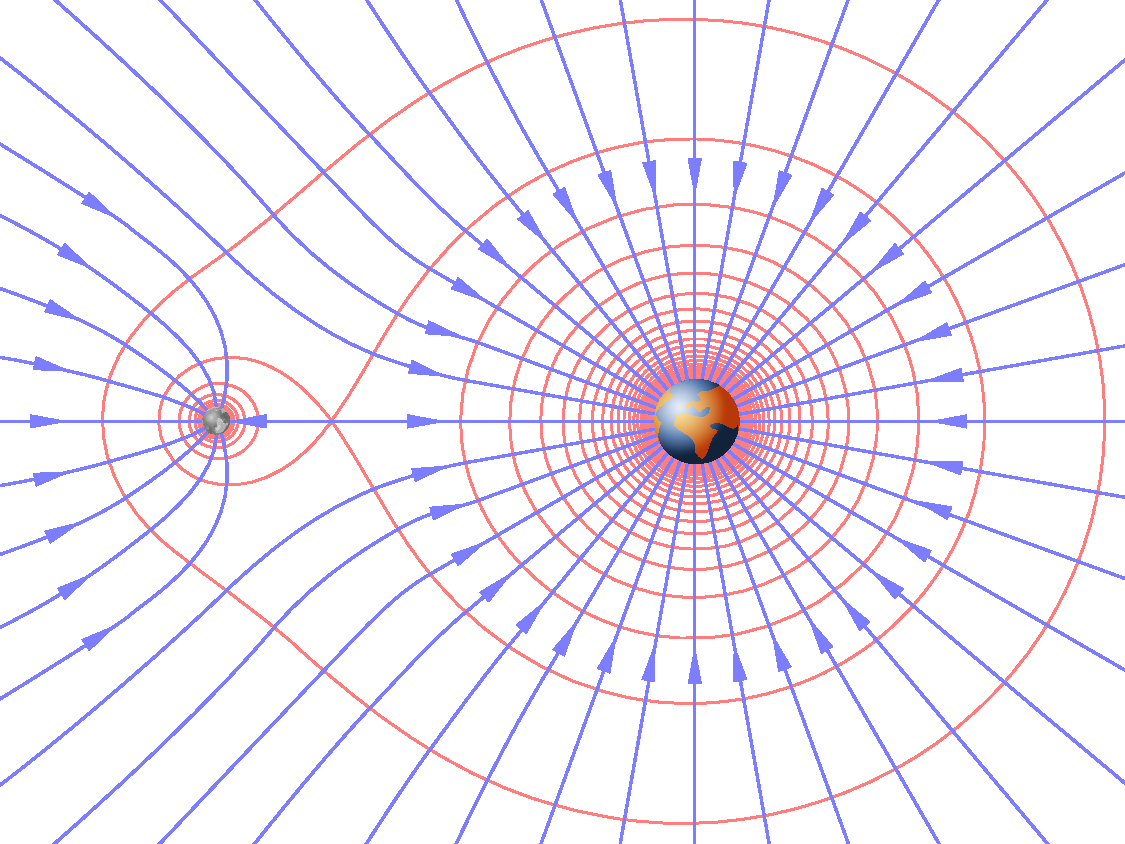
\includegraphics[width=\linewidth]{Pictures/Earth-moon-field.pdf}
    \caption{Lignes de champ et équipotentielles du système Terre-Lune, qui peuvent être calculées via le principe de superposition. Le champ de gravité est plus fort là où les équipotentielles et les lignes de champ sont les plus resserrées. Le champ est le gradient du potentiel, ainsi les lignes de champ et les équipotentielles sont en tout point perpendiculaires. Source : Wikimedia Commons.}
    \label{fig:champ_terre_lune}
\end{figure}


\begin{encart}[Application : le niveau des océans]
    La surface des océans, si on néglige l'existence des courant océaniques, correspond à une surface liquide au repos. Il s'agit donc d'une équipotentielle du champ de gravité terrestre. Cette surface a été cartographiée par satellite et il se trouve qu'elle n'est pas plate du tout (cf figure \ref{fig:geoide}). Ceci est dû au fait que le champ de gravité terrestre n'est pas uniforme, il est plus intense à certains endroits et moins à d'autres.

    En particulier, au voisinage des Antilles, la topographie est complexe en raison du contexte géologique. Une fosse se situe à l'Est de l'arc à cause d'une subduction (la plaque Atlantique passe sous la plaque Caraïbe) et un arc volcanique se trouve au niveau des îles. Les montagnes correspondent à une masse supplémentaire, et cette gravité attire l'eau de l'océan. Au contraire, la fosse correspond à un déficit de masse et la gravité y est moins forte. Conséquence : le niveau de la mer est localement plus élevé au voisinage des îles des petites Antilles, et plus bas à l'Est.

    Ceci ne se voit pas dans les altitudes des cartes topographiques puisque ces altitudes sont calculées à partir du niveau de la mer.
\end{encart}

\begin{figure}
    \centering
    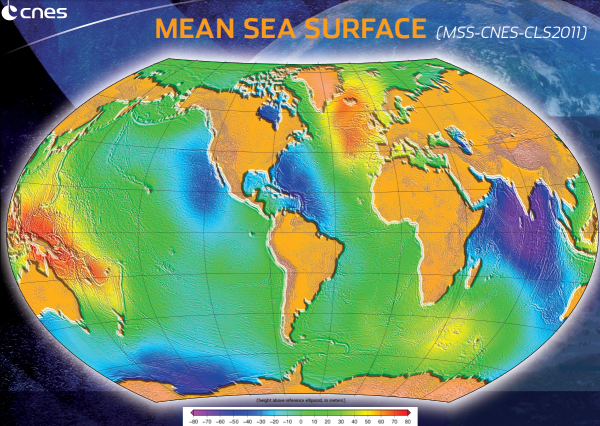
\includegraphics[width=0.75\linewidth]{Pictures/geoid_surface_world.png}
    \caption{Carte de la hauteur de la surface des océans, établie par altimétrie satellite. L'échelle de couleur se mesure en mètres. Source : Centre National d’Études Spatiales (CNES).}
    \label{fig:geoide}
\end{figure}

\begin{figure}
    \centering
    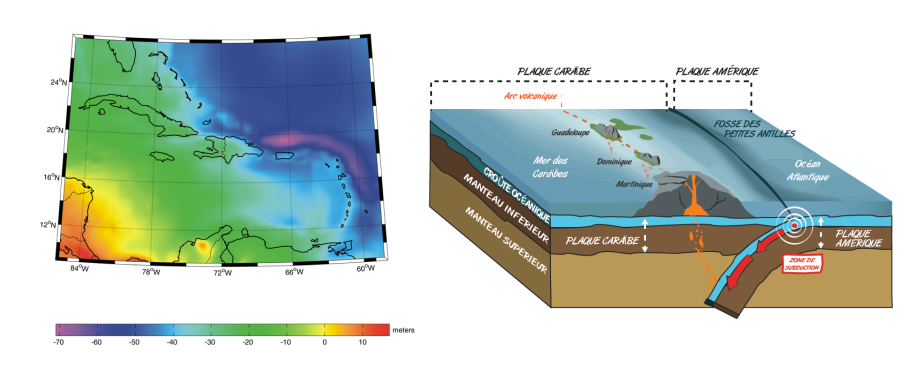
\includegraphics[width=\linewidth]{Pictures/geoid_caribbean.png}
    \caption{Hauteur de la surface des océans dans la région des Antilles. Une coupe géologique et topographique est montrée à droite pour aider l'interprétation de la situation. Sources : International Service for the Geoid et Risques Naturels 972.}
    \label{fig:geoide_caraibes}
\end{figure}

\end{document}
